\documentclass[10pt]{article} 
\usepackage[spanish]{babel}
\usepackage[utf8]{inputenc} 
\usepackage[left=1.50cm, right=1.50cm, top=1.50cm, bottom=1.50cm]{geometry}
\usepackage{blindtext}
\usepackage{multicol}
\usepackage{graphicx}
\usepackage{amsmath}
\usepackage{listings}
\usepackage{xcolor}

\title{Solución numérica de ecuaciones diferenciales de primer orden con valor inicial}
\author{Gustavo Ramos}
\date{7 de Enero 2024}

\definecolor{codegreen}{rgb}{0,0.6,0} 
\definecolor{codegray}{rgb}{0.5,0.5,0.5}
\definecolor{codepurple}{rgb}{0.58,0,0.82} \definecolor{backcolour}{rgb}{0.95,0.95,0.92} 
\lstdefinestyle{mystyle}
{ 
	backgroundcolor=\color{backcolour},
	commentstyle=\color{codegreen}, 
	keywordstyle=\color{magenta}, 
	numberstyle=\tiny\color{codegray}, 
	stringstyle=\color{codepurple}, 
	basicstyle=\ttfamily\footnotesize, 
	breakatwhitespace=true, 
	breaklines,
	captionpos=b,  
	keepspaces=true, 
	numbersep=5pt, 
	showspaces=false, 
	showstringspaces=false, 
	showtabs=false, 
	tabsize=2 
} 
\lstset{style=mystyle}

\begin{document}
	\maketitle
	\begin{abstract}
		Este documento expone dos métodos para resolver ecuaciones diferenciales de primer orden con valor inicial por métodos numéricos, así como la efectividad numérica de cada uno de estos.
	\end{abstract}
	\newpage
	\tableofcontents
	\newpage
	\begin{multicols}{2}
		\section{Introducción}
			Las ecuaciones diferenciales nos han dado un gran avance en temas de ingeniería y ciencias aplicadas, pues nos dan soluciones a problemas diversos, desde el comportamiento de poblaciones, hasta el comportamiento de un tumor maligno, sin embargo, el mayor problema en estas, es que analíticamente, muchas no tienen solución, así que se recurre a los métodos numéricos y a las computadoras para que las resuelvan haciendo uso de estas, siempre con error, pero con el programa correcto, este error puede ser tan pequeño que sera despreciable.
		\section{Antecedentes}
			Las ecuaciones diferenciales ordinarias surgen prácticamente con la aparición del calculo.\\
			El termino $<<$Aequatio Diferentiali$>>$ fue usado principalmente por Leibniz en 1679 para denotar una relación entre las diferenciales $dx$ y $dy$, ademas de las variables $x$ y $y$, esta concepción llega a conservarse hasta los tiempos de Euler.\\
			Otros investigadores afirman que la fecha de aparición de las ecuaciones diferenciales es el 11 de Noviembre de 1675, cuando Leibniz escribió la siguiente ecuación:
			$$\int y \text{ dy}=\frac{y^2}{2}$$
			Se dice por tanto que no fue que resolvió una ecuación diferencial en ese entonces, sino que fue un acto donde se vio Leibniz ideando el signo de la integral.\\
			En la ultima década del siglo XVII los hermanos Bernoulli introducen términos como el de integrar una ecuación diferencial, asimismo formalizan el proceso de separación de variables.\\
			En 1692 Johan Bernoulli formula otro método utilizando una serie de problemas, la multiplicación por un factor integrante.\\
			En 1768, Euler publica $<<$Instituciones$>>$ que es la primera teoría de las ecuaciones diferenciales ordinarias.\\
			D' ALembert en 1766 dio la solución general de una ecuación diferencial no homogénea, en 1774, Lagrange demostró el principio de superposición y la variación de parámetros.\\
			Para le siglo XIX fue la fase en la que se demostraron los hechos dados por ciertos en los siglos anteriores, como la existencia de una solución a la ecuación $x(t)'=f(t,x)$ (Cauchy 1820).
		\section{Metodología}
			\subsection{Ecuación diferencial ordinaria de primer orden}
				Las ecuaciones diferenciales de primer orden son aquellas de la forma:
				$$y'=f(x,y)$$
				Sin embargo, para una función arbitraria $f$, no existe un método general para resolver esta ecuacion en términos de funciones elementales. En lugar de ello, se describen varios métodos, cada uno de los cuales es aplicable a ciertas subclase de ecuaciones.\\
				Para estas ecuaciones, cualquier función diferencial $y\phi(x)$ que satisface la ecuacion para $x$ en algún intervalo, se llama solución de la ecuacion, y para cada ecuación de primer orden, siempre existe una solución.
			\subsection{Error por truncamiento}
				Al resolver numericamente un problema con valor inicial, existen dos fuentes de error fundamentales. En primer lugar, supóngase que la computadora con la que se cuenta es capaz de efectuar todos los calculos con completa exactitud; es decir, es posible retener una infinidad de cifras decimales. La diferencia $E_n$ entre la solución exacta $y=\phi(x)$ y la solución aproximada del problema con valor inicial se expresa por:
				$$E_n=\phi(x_n)-y_n$$
				y se conoce como error global por truncamiento. Este error surge por dos causas: $1)$ en cada paso se aplica una formula aproximada para determinar $Y_{n+1}$; $2)$ los datos de entrada en cada caso no concuerdan con la solución exacta ya que, en general, $\phi(x_n)$ no es igual a $y_n$. Si se supone que los datos de entrada son correctos, entonces el único error al avanzar un paso se debe al uso de una formula aproximada. Este error se denomina error local por truncamiento $e_n$. 
			\subsection{Método de Euler}
				Con el método de Euler es posible hallar en el segmento $[x_o,b]$ la solución aproximada a la ecuación $y'=f(x,y)$ que satisface a la condición inicial $y(x_o)=y_o$.\\
				El método de Euler consiste en sustituir por una quebrada de segmentos rectos la curva integral buscada de la ecuación diferencial que pasa por el punto $M_o(x_o,y_o)$.\\
				Dividamos el segmento $[x_o,b]$ en $n$ partes (no necesariamente iguales) por los puntos $x_o<x_1<x_2<\dots<x_n=b$.\\
				Tracemos por el punto inicial $M_o$ de la curva integral, una recta $M_oM$ de coeficiente angular $f(x_o,y_o)$, hasta el punto $M_1(x_1,y_1)$ de intersección con la recta $x=x_1$. La ordenada del punto $M_1$ se determina por la formula:
				$$y_1=y_o+f(x_o,y_o)(x_1-x_o)$$
				Hacemos lo mismo desde $M_1$ hasta $M_2$ de coeficiente angular $f(x_1,y_1)$. La ordenada del punto $M_2$ se determina por la formula:
				$$y_2=y_1+f(x_1,y_1)(x_2-x_1)$$
				Y repetimos hasta el punto $M_n$, obteniendo que:
				$$y_n=y_{n-1}+f(x_{n-1},y_{n-1})(x_n-x_{n-1})$$
				Así, los valores aproximados para los puntos $x_i$ son $y_i$ con $i=1,2,\dots,n$.\\
				Generalmente, para facilitar los cálculos y las acotaciones, se divide el segmento $[x_o,b]$ en partes iguales y se hace la notación $h=x_k-x_{k-1}$. La magnitud $h$ se llama intervalo de variación del argumento.\\
				Se puede demostrar que cumpliéndose ciertas condiciones respecto de la función $f(x,y)$, para $h\to 0$ la solución aproximada proporciona la solución exacta de la ecuacion dada que satisface la condición inicial $y(x_o)=y_o$
			\subsection{Método de Runge-Kutta}
				Nuevamente, para el problema con valor inicial:
				$$y'=f(x,y),\text{		}y(x_o)=y_o$$
				El error local por truncamiento de este método es proporcional a $h^5$.\\
				La formula de Runge-Kutta comprende un promedio ponderado de valores $f(x,y)$ tomados en diferentes puntos del intervalo $x_n\leq x\leq x_{n+1}$; se expresa por:
				$$y_{n+1}=y_n+\frac{h}{6}\left( k_{n1}+2k_{n2}+2k_{n3}+k_{n4} \right)$$
				en donde:
				\begin{equation*}
					\begin{split}
						&k_{n1}=f(x_n,y_n)\\
						&k_{n2}=f\left(x_n+\frac{1}{2}h,y_n+\frac{1}{2}hk_{n1}\right)\\
						&k_{n3}=f\left(x_n+\frac{1}{2}h,y_n+\frac{1}{2}hk_{n2}\right)\\
						&k_{n4}=f(x_n+h,y_n+hk_{n3})
					\end{split}
				\end{equation*}
				Donde la suma de las $k_{ni}$ entre 6 puede interpretarse como una pendiente promedio.\\
				El desarrollo de las variables $k_{ni}$ resultan del desarrollo en serie de Taylor de la función $\phi(x)$ hasta un termino $h^5$.\\
				Nótese que si la función $f$ no depende de $y$, la relación de recurrencia se reduce a:
				$$y_{n+1}-y_n=\frac{h}{6}\left[ f(x_n)+4f(x_n+h/2)+f(x_n+h) \right]$$
				que la hemos visto anteriormente, es la regla de Simpson.
		\section{Análisis y resultados}
			\subsection{Solución a 10 ecuaciones diferenciales}
				Dadas 10 ecuaciones diferenciales con condición inicial y(0)=1, sus respectivas soluciones numéricas por ambos métodos se muestran en el siguiente apartado e inmediatamente después, la diferencia numérica entre ambas soluciones.\\
		\subsection{Resultados}
			1.- $y'=y^2-x^3+1$
			\begin{center}
				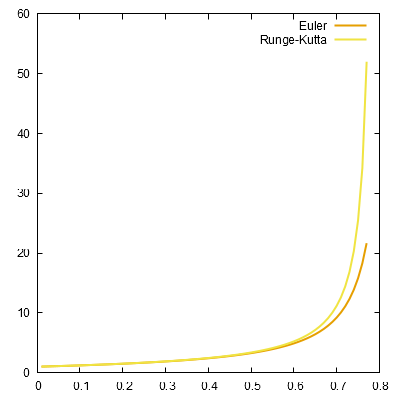
\includegraphics[scale=0.4]{../Graficas/1.png}
			\end{center}
			\begin{center}
				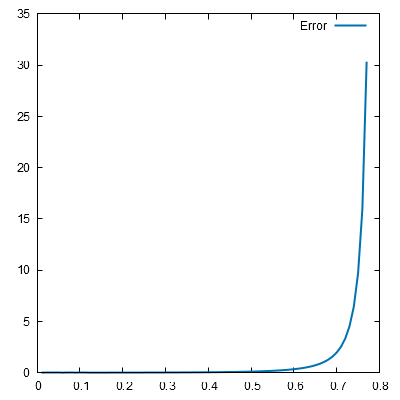
\includegraphics[scale=0.4]{../Graficas/1_1.png}
			\end{center}
			2.- $y'=y^3-5x+2$
			\begin{center}
				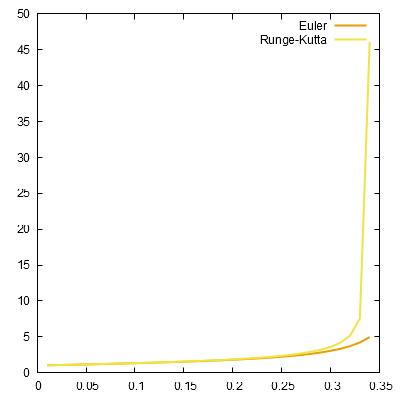
\includegraphics[scale=0.4]{../Graficas/2.png}
			\end{center}
			\begin{center}
				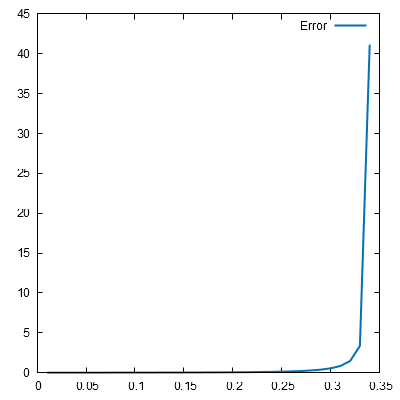
\includegraphics[scale=0.4]{../Graficas/2_1.png}
			\end{center}
			3.- $y'=3y^2+\cos(x)$
			\begin{center}
				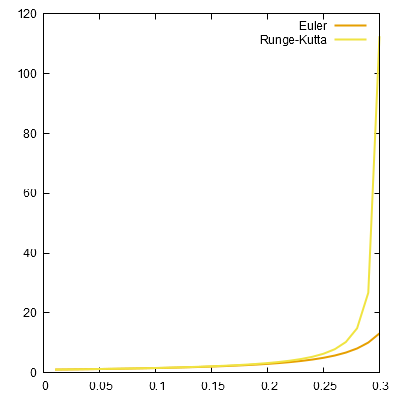
\includegraphics[scale=0.4]{../Graficas/3.png}
			\end{center}
			\begin{center}
				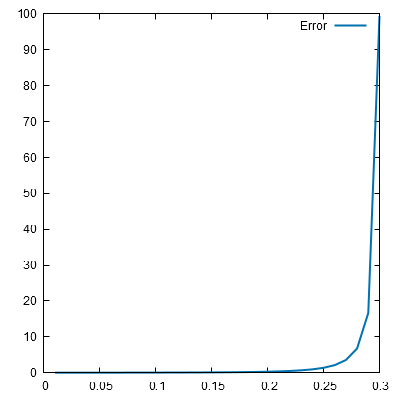
\includegraphics[scale=0.4]{../Graficas/3_1.png}
			\end{center}
			4.- $y'=4y^4+4y+4$
			\begin{center}
				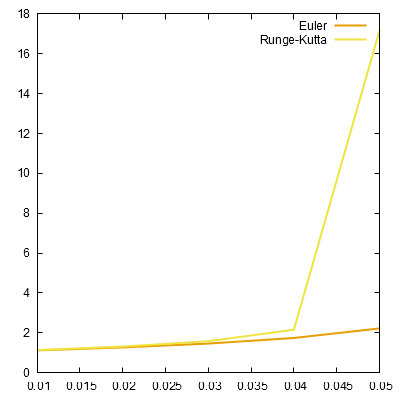
\includegraphics[scale=0.4]{../Graficas/4.png}
			\end{center}
			\begin{center}
				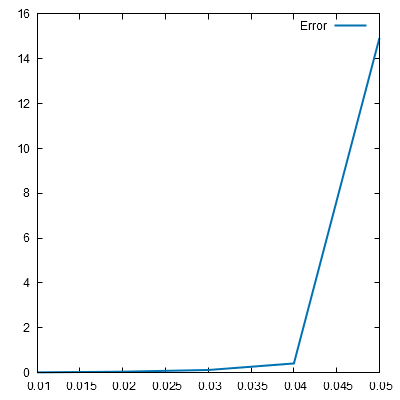
\includegraphics[scale=0.4]{../Graficas/4_1.png}
			\end{center}
			5.- $y'=-3y+\sin(x)-2$
			\begin{center}
				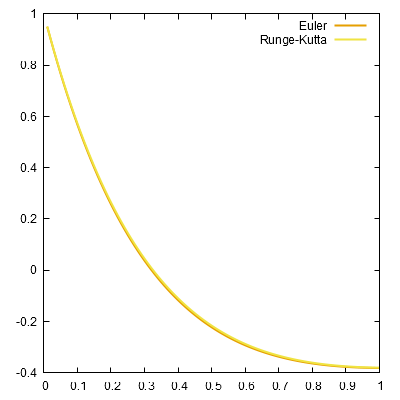
\includegraphics[scale=0.4]{../Graficas/5.png}
			\end{center}
			\begin{center}
				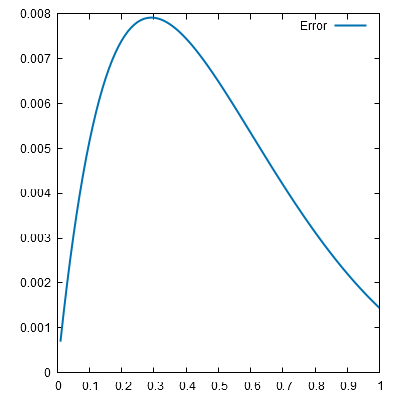
\includegraphics[scale=0.4]{../Graficas/5_1.png}
			\end{center}
			6.- $x'=\cos(x^2)+5y-4$
			\begin{center}
				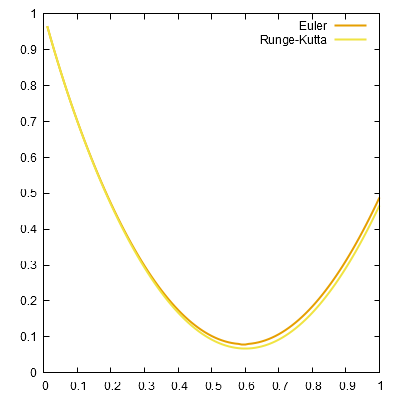
\includegraphics[scale=0.4]{../Graficas/6.png}
			\end{center}
			\begin{center}
				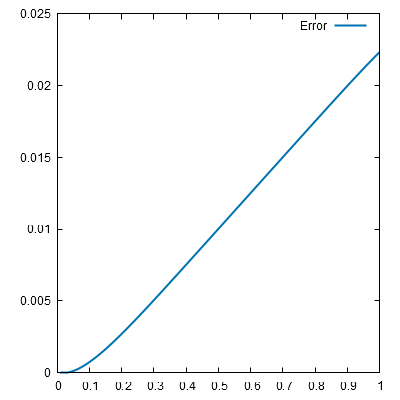
\includegraphics[scale=0.4]{../Graficas/6_1.png}
			\end{center}
			7.- $x'=1/2x^3-2/3$
			\begin{center}
				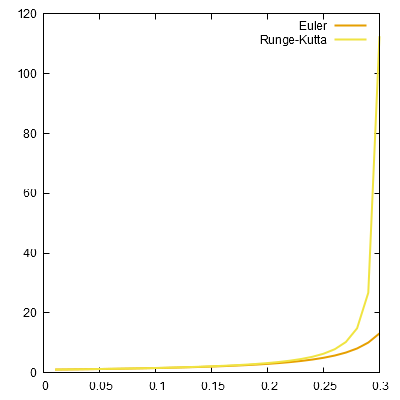
\includegraphics[scale=0.4]{../Graficas/7.png}
			\end{center}
			\begin{center}
				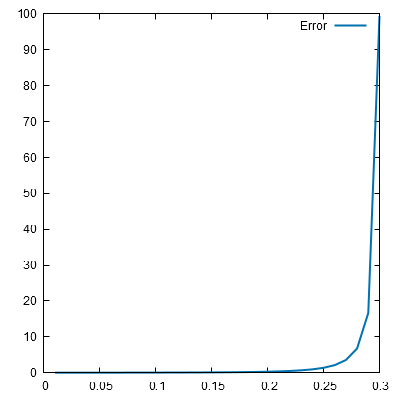
\includegraphics[scale=0.4]{../Graficas/7_1.png}
			\end{center}
			8.- $x'=x^3-y^2+2$
			\begin{center}
				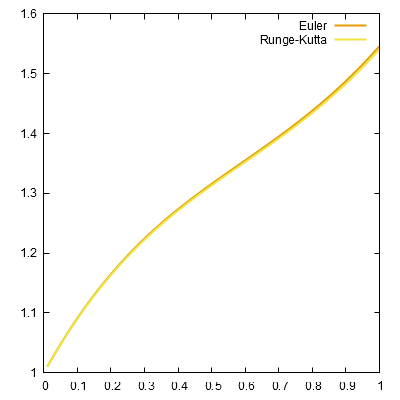
\includegraphics[scale=0.4]{../Graficas/8.png}
			\end{center}
			\begin{center}
				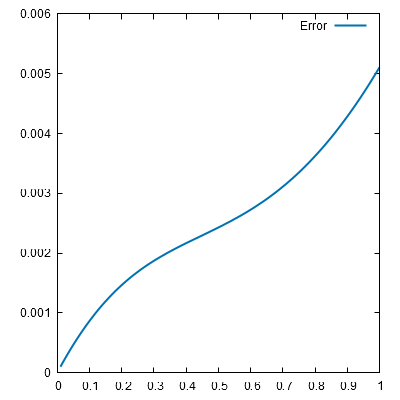
\includegraphics[scale=0.4]{../Graficas/8_1.png}
			\end{center}
			9.- $x'=-2sin(x)+y^3$
			\begin{center}
				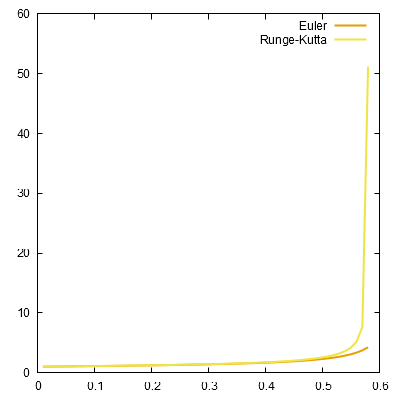
\includegraphics[scale=0.4]{../Graficas/9.png}
			\end{center}
			\begin{center}
				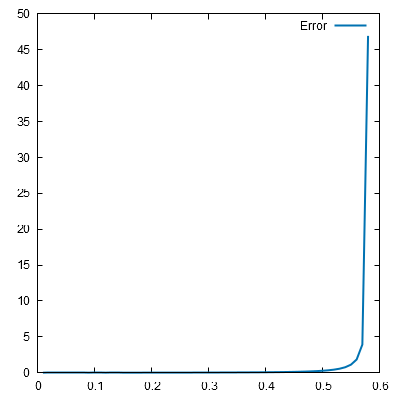
\includegraphics[scale=0.4]{../Graficas/9_1.png}
			\end{center}
			10.- $5x^2+3y-2$
			\begin{center}
				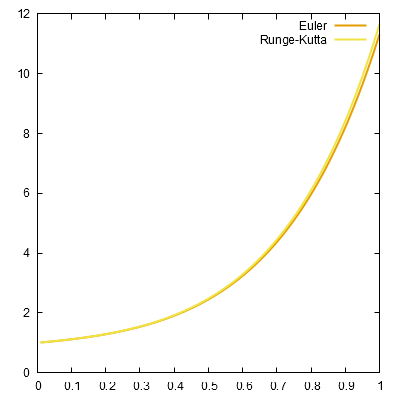
\includegraphics[scale=0.4]{../Graficas/10.png}
			\end{center}
			\begin{center}
				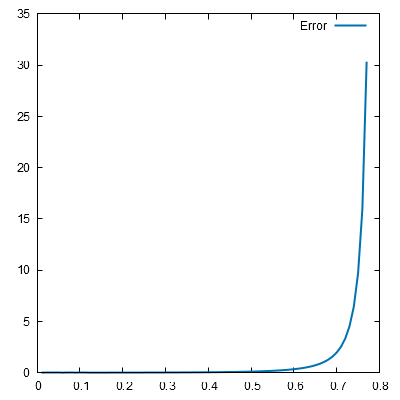
\includegraphics[scale=0.4]{../Graficas/1_1.png}
			\end{center}
		\section{Conclusiones}
			El método de Euler es numéricamente impreciso comparado con el de Runge-Kutta, y para igualarlo, el método de Euler tendría que hacer diez veces los pasos que se hacen con el método de Runge-Kutta y aun así tendría errores altos.
	\end{multicols}
	\appendix 
	\section{Diseño del código}
		\subsection{Método de Euler}
			\lstinputlisting[language=c]{../Euler.c}
		\subsection{Método de Runge-Kutta}
			\lstinputlisting[language=c]{../RK.c}
		\subsection{Ecuaciones diferenciales}
			\lstinputlisting[language=c]{../funciones.h}
	\begin{multicols}{2} 
		\section{Referencias} 
		$[1]$ Boyce, W. and DiPrima, R., 2013. Ecuaciones diferenciales y problemas con valores en la frontera. 4th ed. México, D.F.: Limusa.\\\\
		$[2]$ Kiseliov, A., Kiseljak, M. and Makarenko, G., 1973. Problemas de ecuaciones diferenciales ordinarias. Moscow: MIR.\\\\
		$[3]$ Napoles, Juan y Segura, Carlos. $<<$Historia de las Ecuaciones Diferenciales$>>$ Revista Electronica. Universidad de la Cuenca del Plata. Argentina. Año 3, Numero 2. Octubre 2002. Disponible en: uaq.mx/matematicas/redm
		
	\end{multicols} 
\end{document}